\section{Motivating Example}
\label{sec:optics}

\begin{wrapfigure}{r}{.4\textwidth}
\vspace{-20pt}
\centering
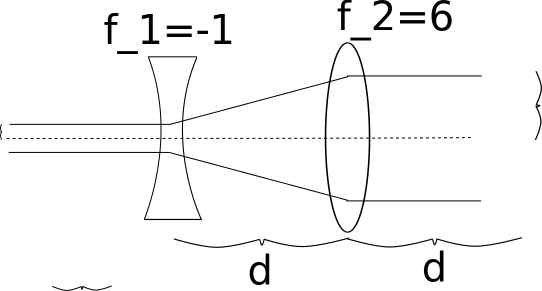
\includegraphics[width=.5\textwidth]{images/beam_expander}
\vspace{-0pt}
\caption{A simple beam expander}
\label{fig:beam_expander}
\vspace{-10pt}
\end{wrapfigure}

To motivate the use of random expressions we build a simple example. Consider the beam expander depicted in figure \ref{fig:beam_expander}. It consists of a thin concave lens of focal length $f_1$, followed by $d$ units of free space, followed by a convex lens of focal length $f_2$, followed by $d$ more units of free space followed by a target. If $f_2 = d-f_1$ then incoming parallel horizontal rays produce outgoing parallel rays. I.e. beams remain beams though their widths may
expand or contract.

If we allow only rays with small angles then such systems can be concisely described using matrices. We build such a system in using the built-in SymPy Gaussian optics module. 

\begin{lstlisting} 
f1 = Symbol('f1')
f2 = Symbol('f2')
d = Symbol('d')

lens1 = optics.ThinLens(f1)
lens2 = optics.ThinLens(f2)
space = optics.FreeSpace(d)

beam_expander = space*lens2*space*lens1

height = 5
angle = 0
ray = optics.GeometricRay(height, angle)

exit_ray = beam_expander * ray
exit_height, exit_angle = exit_ray

\end{lstlisting} 

If we substitute in values $f_1 = -1 , d=5 , f_2=6$ we find that the exit height equals 30, magnified six times, while the exit angle remains 0. 

We now consider a more realistic setting where the device to set the ray's angle has some normally distributed error. In this example we describe te ray's angle with mean zero and standard deviation $pi/100$.

\begin{lstlisting}
angle = Normal(0, pi/100)
\end{lstlisting}

\code{angle} is an object of the RandomSymbol type. It acts like as a SymPy Symbol (like \code{d}, \code{f1}, and \code{f2}) in most situations. Our previous code still produces an expression for the exit height and angle of the beam and need not be changed to incorporate this new statistical information.

\begin{lstlisting}
ray = optics.GeometricRay(height, angle)
exit_ray = beam_expander * ray
exit_height, exit_angle = exit_ray
\end{lstlisting}
$$ \texttt{exit\_ray} = \left[\begin{smallmatrix}\frac{\theta d \left(- d + 2 f_{2}\right)}{f_{2}} - 5 \frac{d}{f_{2}} + 5 - 5 \frac{d \left(- \frac{d}{f_{2}} + 1\right) + d}{f_{1}}\\\frac{\theta \left(- d + f_{2}\right)}{f_{2}} + 5 \frac{d - f_{1} - f_{2}}{f_{1} f_{2}}\end{smallmatrix}\right]$$

or, given $f_1=-1, d = 5, f_2 = 6$

$$ \texttt{exit\_ray} = \left[\begin{smallmatrix}\frac{35}{6} \theta + 30\\\frac{1}{6} \theta\end{smallmatrix}\right]$$ 
Because these symbolic SymPy expressions contain RandomSymbols the are now random expressions and support the action of special statitical query functions such as...
\begin{itemize}
\item The expectation and variance.  \\
\indent \code{E(exit\_height)} $ = 30 $\\
\indent \code{var(exit\_height)} $ = 0.0335840705314846$

\item The full probability density.\\ 
\indent \code{Density(exit\_height)} $ = \frac{60}{7} \frac{\sqrt{2} e^{- 5000 \frac{\left(\frac{6}{35} z - \frac{36}{7}\right)^{2}}{\pi^{2}}}}{\pi^{\frac{3}{2}}}$

\item Or even direct questions about specific conditions that may be pertinent to the problems at hand. \\
\indent \code{P(exit\_height>30.2)} $ = 0.137559852249536$
\end{itemize}
